%OBAL
\thispagestyle{empty}
\begin{center}
  \textsc{ 
    {\Large \school\\ \faculty}
    \vfill
    {\LARGE \title}\\ \vspace{0.5cm}
    {\large \thesis}
  }
\end{center}
\vfill

\begin{flushleft}
  \year\\
  \hspace{0.5cm} \author
\end{flushleft}


%TITULNY LIST
\thispagestyle{empty}
\begin{center}
  \textsc{ 
    {\Large \school\\ \faculty}
    \vfill
    {\LARGE \title}\\ \vspace{0.5cm}
    {\large \thesis}
  }
\end{center}
\vfill

\begin{flushleft}
  \begin{tabular}{@{}ll}
    Študijný program: & \studyprogramme \\
    Odbor: & \studyfield \\
	Katedra: & \department \\
    Vedúci: & \supervisor
  \end{tabular}
  \vspace{1cm}

  \placeandyear\\
  \hspace{0.5cm} \author
\end{flushleft}



\shorthandoff{-} %docasne deaktivuje znak '-' v balicku babel
%ZADANIE EN
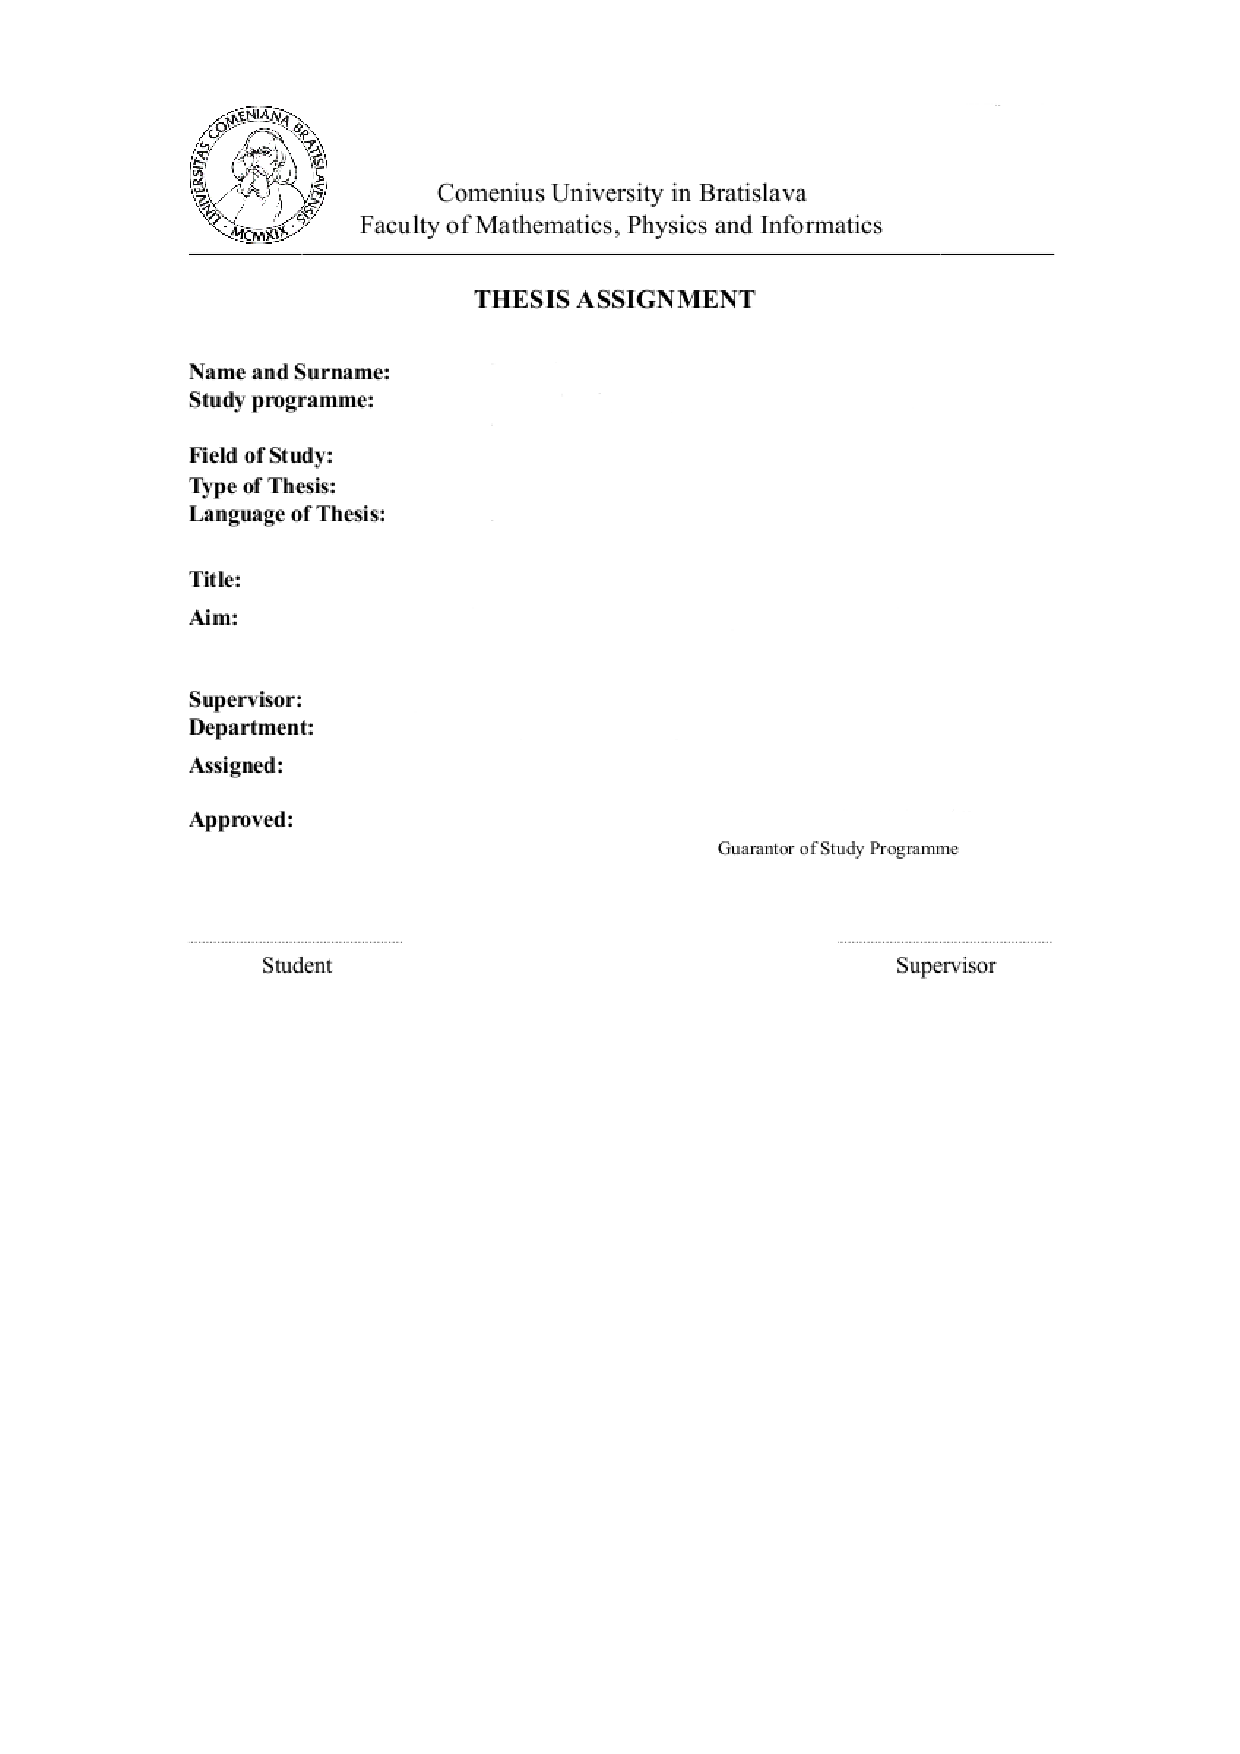
\includepdf[pages=-]{frontmatter/assignment.pdf}
%ZADANIE SK
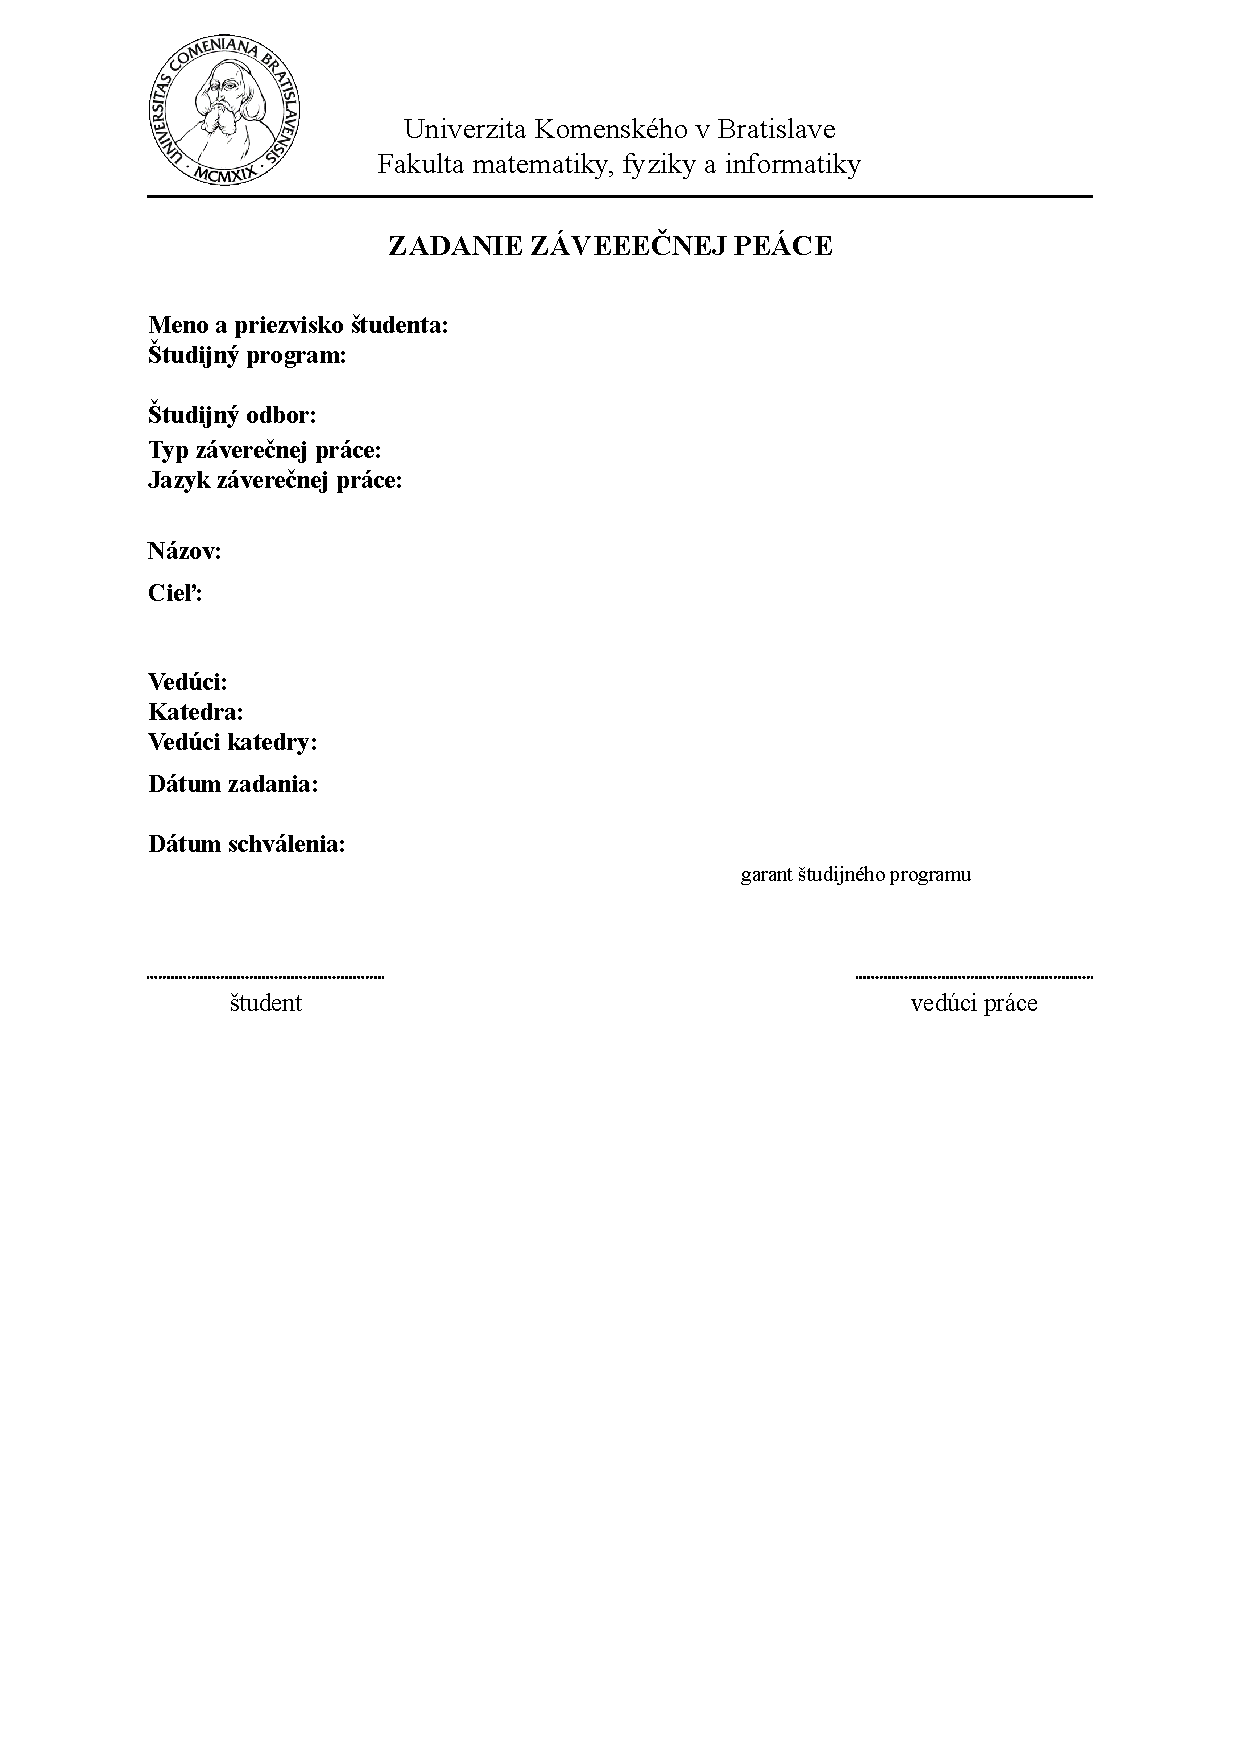
\includepdf[pages=-]{frontmatter/zadanie.pdf}
\shorthandon{-}

%PODAKOVANIE
\chapter{Poďakovanie}
\vfil
Týmto by som sa chcel poďakovať svojmu vedúcemu Mgr. Marekovi Zemanovi za podnetné nápady, rady a odbornú spoluprácu, katedre informatiky, predovšetkým Mgr. Jaroslavovi Budišovi za poskytnutie prostriedkov na vykonanie potrebných výpočtov a rodine a priateľom za podporu.


%ABSTRAKT SK
\selectlanguage{slovak}
\chapter{Abstrakt}
Lorem Ipsum je fiktívny text, používaný pri návrhu tlačovín a typografie. Lorem Ipsum je štandardným výplňovým textom už od 16. storočia, keď neznámy tlačiar zobral sadzobnicu plnú tlačových znakov a pomiešal ich, aby tak vytvoril vzorkovú knihu. Prežil nielen päť storočí, ale aj skok do elektronickej sadzby, a pritom zostal v podstate nezmenený. Spopularizovaný bol v 60-tych rokoch 20. storočia, vydaním hárkov Letraset, ktoré obsahovali pasáže Lorem Ipsum, a neskôr aj publikačným softvérom ako Aldus PageMaker, ktorý obsahoval verzie Lorem Ipsum.\\ \\
\textbf{\textsc{Kľúčové slová:}} lorem, ipsum, consectetur


%ABSTRAKT EN
\chapter{Abstract}
The topic of this bachelor thesis is to analyze the deterministic and non deterministic state complexity of regular languages, focusing on the automata over binary alphabet. An important part of this thesis are the chapters 4 and 5, where we present our results. Also the attached program, through which we computed the results.
\textbf{\textsc{Keywords:}} finite automata, minimal NFA, minimal DFA, state complexity, enumeration of regular languages


%PREDHOVOR
%\selectlanguage{english}
%input{frontmatter/preamble}

%OBSAH
\tableofcontents

%ZOZNAM ILUSTRACII
\listoffigures

%ZOZNAM TABULIEK
\listoftables
